\chapter{Solution approach of an automated EAD process}\label{chapter:approach}

This chapter will propose a new automated process for EAD derived from the lack of integrating cloud infrastructure for automated EA documentation in the context of agile methodologies and continuous delivery and integration. The proposed approach was derived from the topics that are not covered and the requirements derived from the already existing approaches in section~\ref{chapter:relatedwork}.

The first section~\ref{section:solution-architecture} will give an overview of the solution architecture. The second section~\ref{section:approach-ead} will describe how to automate the EAD from the application development pipeline and what requirements need to be fulfilled. The last section~\ref{section:approach-usage-scenario} will describe the process more in detail showing the approach in a sample scenario with common tools.

%How  to  assign  the  application  landscape  to  business  domains?
%How  to  obtain  EA  relevant  information  from  the  runtime  behaviour  of cloud-based environments?
%How to automate the assignment process with an integrated toolchain?
%How  does  a  prototype  implementation  of  the  automated  documentation process of cloud applications look like?
\section{Solution architecture}\label{section:solution-architecture}

Driven by the requirements of the literature and the deficiency of automated EAD approaches for cloud infrastructures, the following solution was developed.

Figure~\ref{fig:solution-architecture-general} shows the solution architecture of the automated EAD solution. 

The components that are content of this work are:
\begin{itemize}
    \item A cloud infrastructure
    \item A Version control service
    \item A PPM Tool
    \item A CD/CI Tool
    \item A EA Tool
\end{itemize}

%bild mit tools. (generel)
\begin{figure}[htpb]
  \centering
  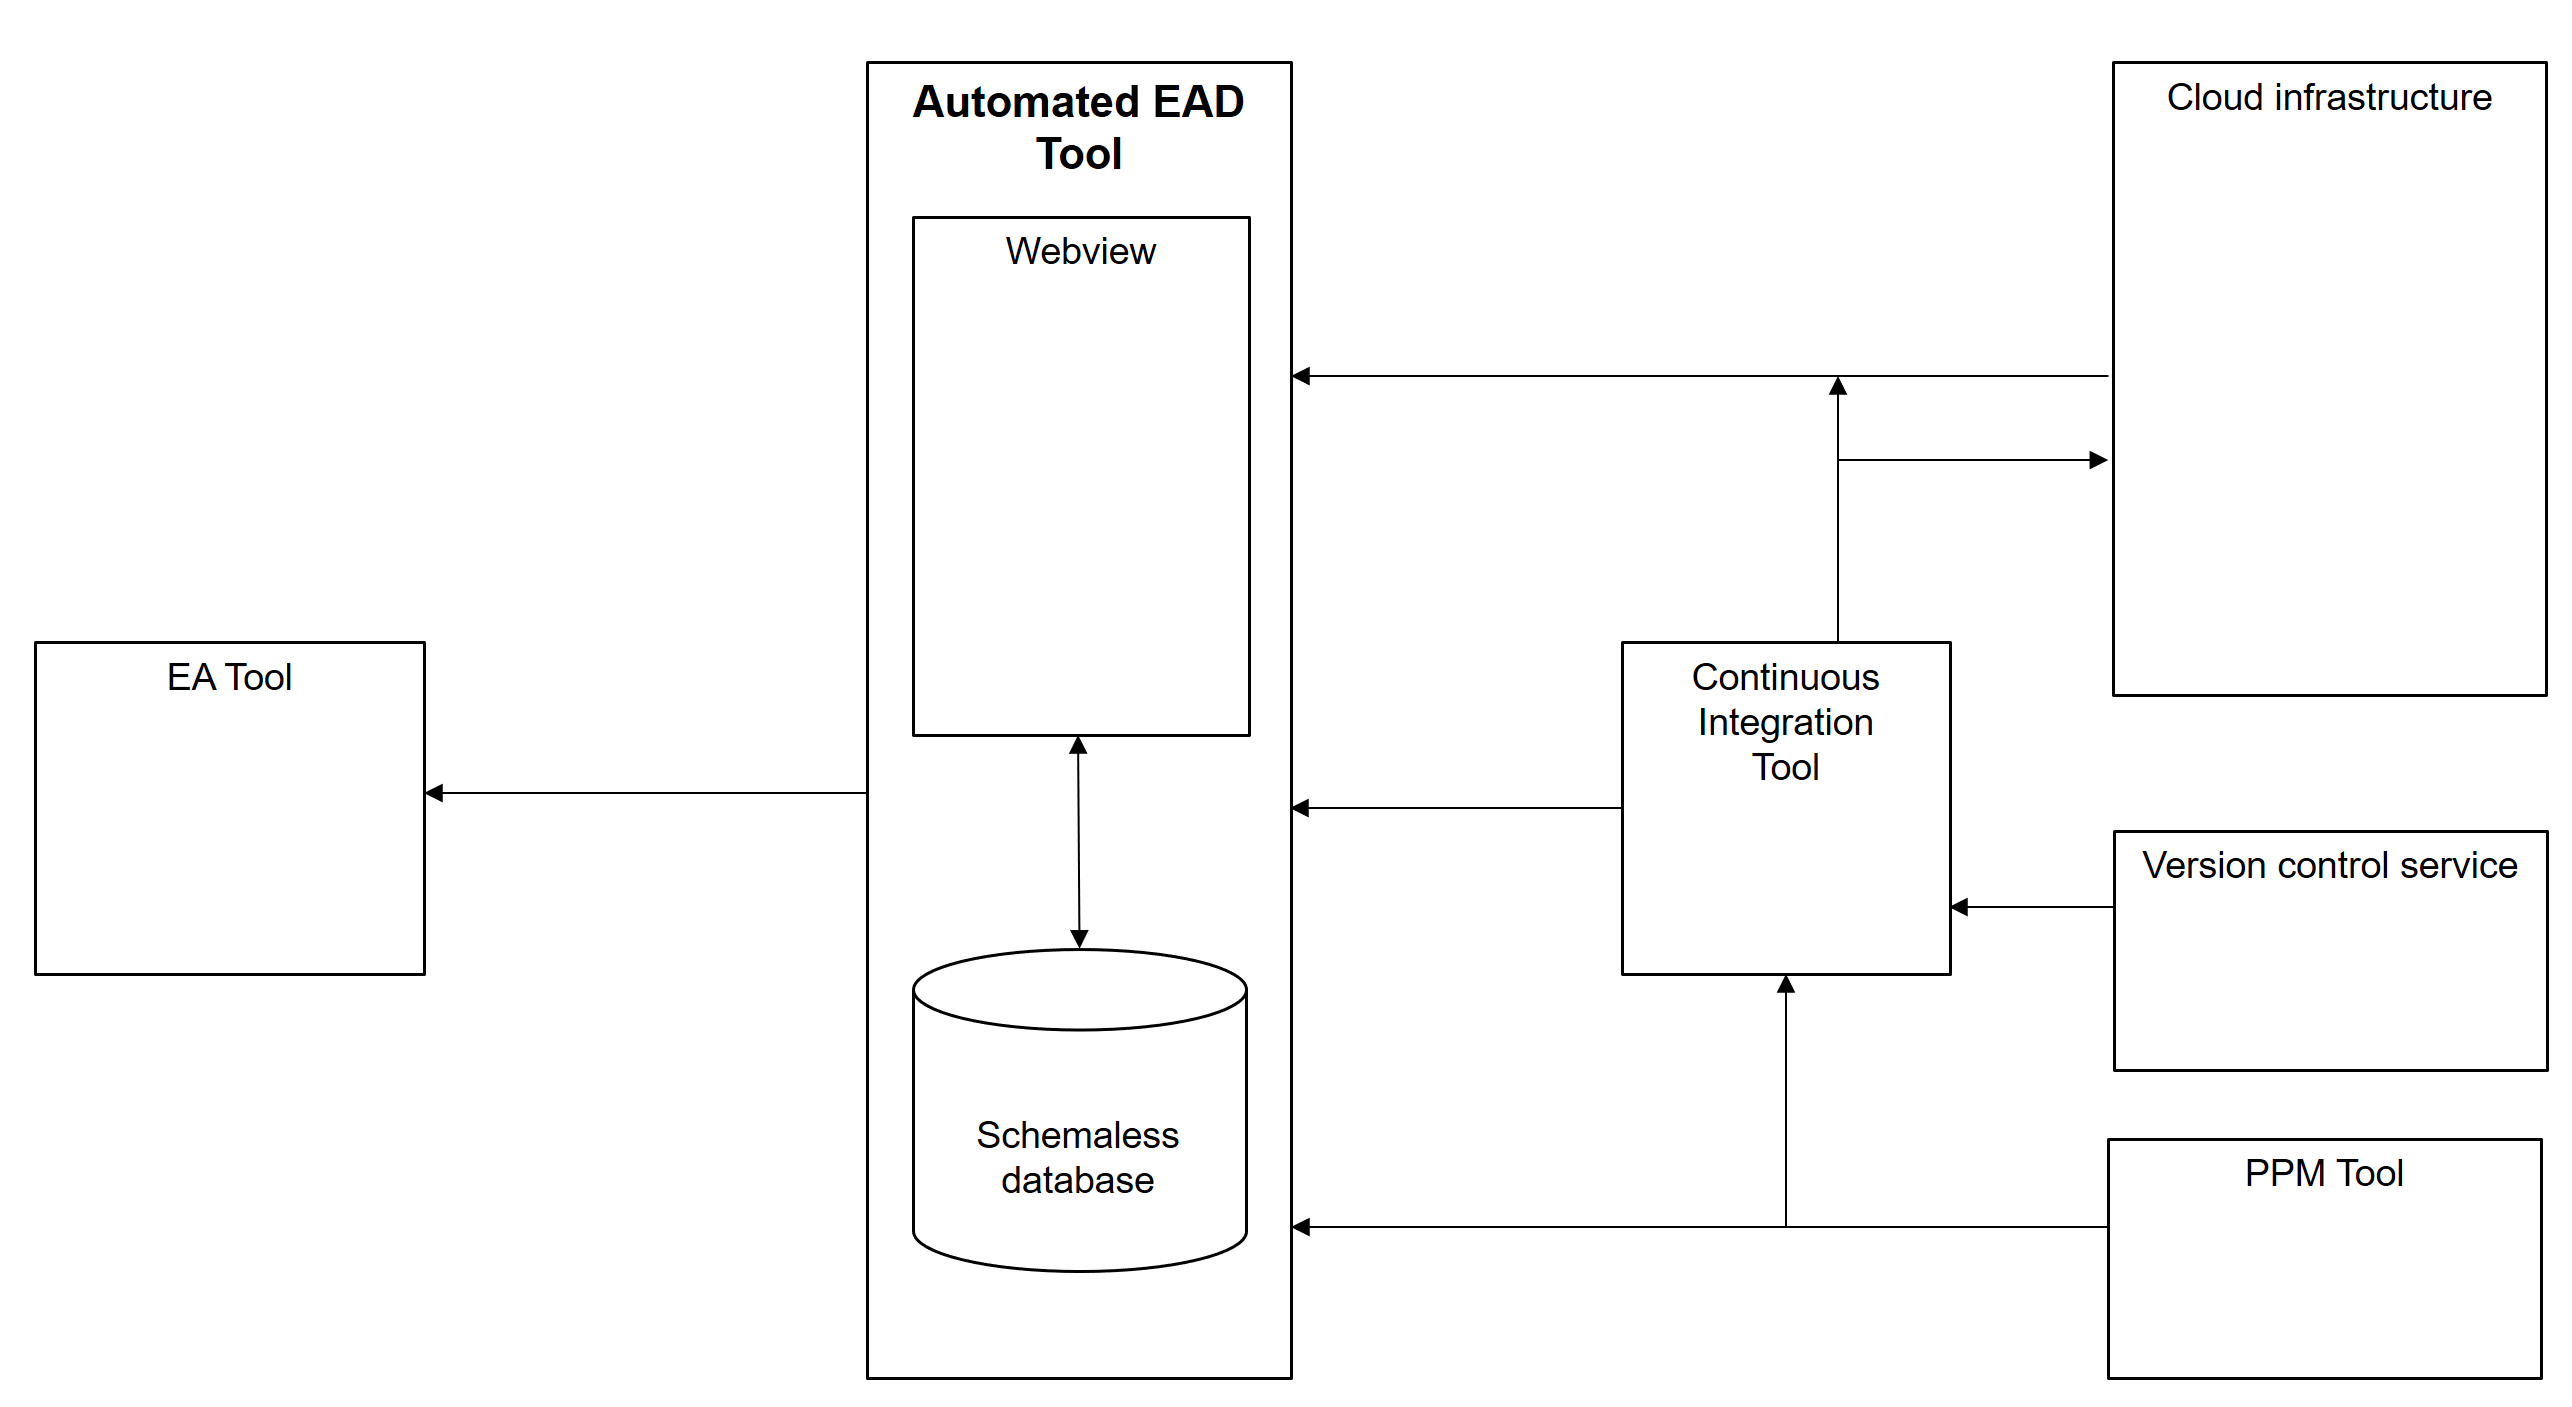
\includegraphics[width=1.0\textwidth]{figures/solution-architecture-general.PNG}
  \caption{Solution architecture}
  \label{fig:solution-architecture-general}
\end{figure}

The prototypical implementation for for this approach is illustrated in figure~\ref{fig:solution-architecture-general} as "Automated EAD Tool". It is integrated as a middle layer to aggregate the information of the components mentioned above since many of the existing EA Tools require a lot of effort to integrate different information sources. An adaption of the EA metamodel within the EA tool is still an intensive process. Therefore the automated EAD tool as  a middlelayer is useful to aggregate the different collected content.

The main reason for an integration of a PPM Tool is to enable the assignment of the application landscape to the business domains asked in \textbf{RQ1}. The PPM tool maintain and ensure the business-specific information like business domains, subdomains and product assignments to aggregate the information to the application. The Product Owner should ensure that the project of the PPM tool contains this information. The involvement of data owners is needed to ensure a complete EAD. Therefore the product owner should have the responsibility to maintenance this EA relevant information.

To obtain EA relevant information from the runtime-behavior (\textbf{RL6}) of cloud-based environments asked in \textbf{RQ2} an integration of the cloud infrastructure is required (\textbf{RL5}). The goal of the integration of the cloud infrastructure is to identify how to obtain runtime information of applications running in a cloud-based environments and what information is relevant for EAM. 

CD/CI Tools and VCS can automate build and deployment processes. As described by Chen et al. and by Drews et al. DevOps teams do not document small changes in the application development pipeline. Thus a documentation process can be integrated in the pipeline with no effort to automate the EAD and improve the data quality attributes mentioned in table~\ref{tab:data-challenges} Therefore an integration of the application development pipeline and the according tools are content of this work to automate the documentation and assignment process.

The proposed solution is structured in two main parts:
\begin{itemize}
    \item A Webview
    \item A schemaless database with a REST API
\end{itemize}

The integration of different information sources required in \textbf{RL1} and that are of relevance for this approach, are the cloud infrastructure a VCS, a CD/CI tool and the PPM tool. The collection of the relevant information of this sources is achieved due to a REST API layer connected to the database.

Many of the approaches request a dynamic metamodel. A possible solution to a dynamic metamodel are required in \textbf{RL2} is the usage of a schemaless database. A schemaless database enables the storage of structured and unstructured data since it does not require a static and predefined schema and allows the integration of different granularity levels (DC1).

An aggregated information consisting of the runtime information and the business domain assigments can be exported from the prototypical implementation to the EA Tool if the tool supports a data integration through an API: \textbf{RL4}.

%Automated documentation of Business Domain assignments and cloud application information from an application development pipeline
\section{Approach for an automated documentation}\label{section:approach-ead}

This section introduces an automated EAD process.The focus of this work is the process of an automated EAD from an application development pipeline. The process is described in subsection~\ref{subsection:processdescription}.

%bild mit sprzifischen tools
\begin{figure}[htpb]
  \centering
  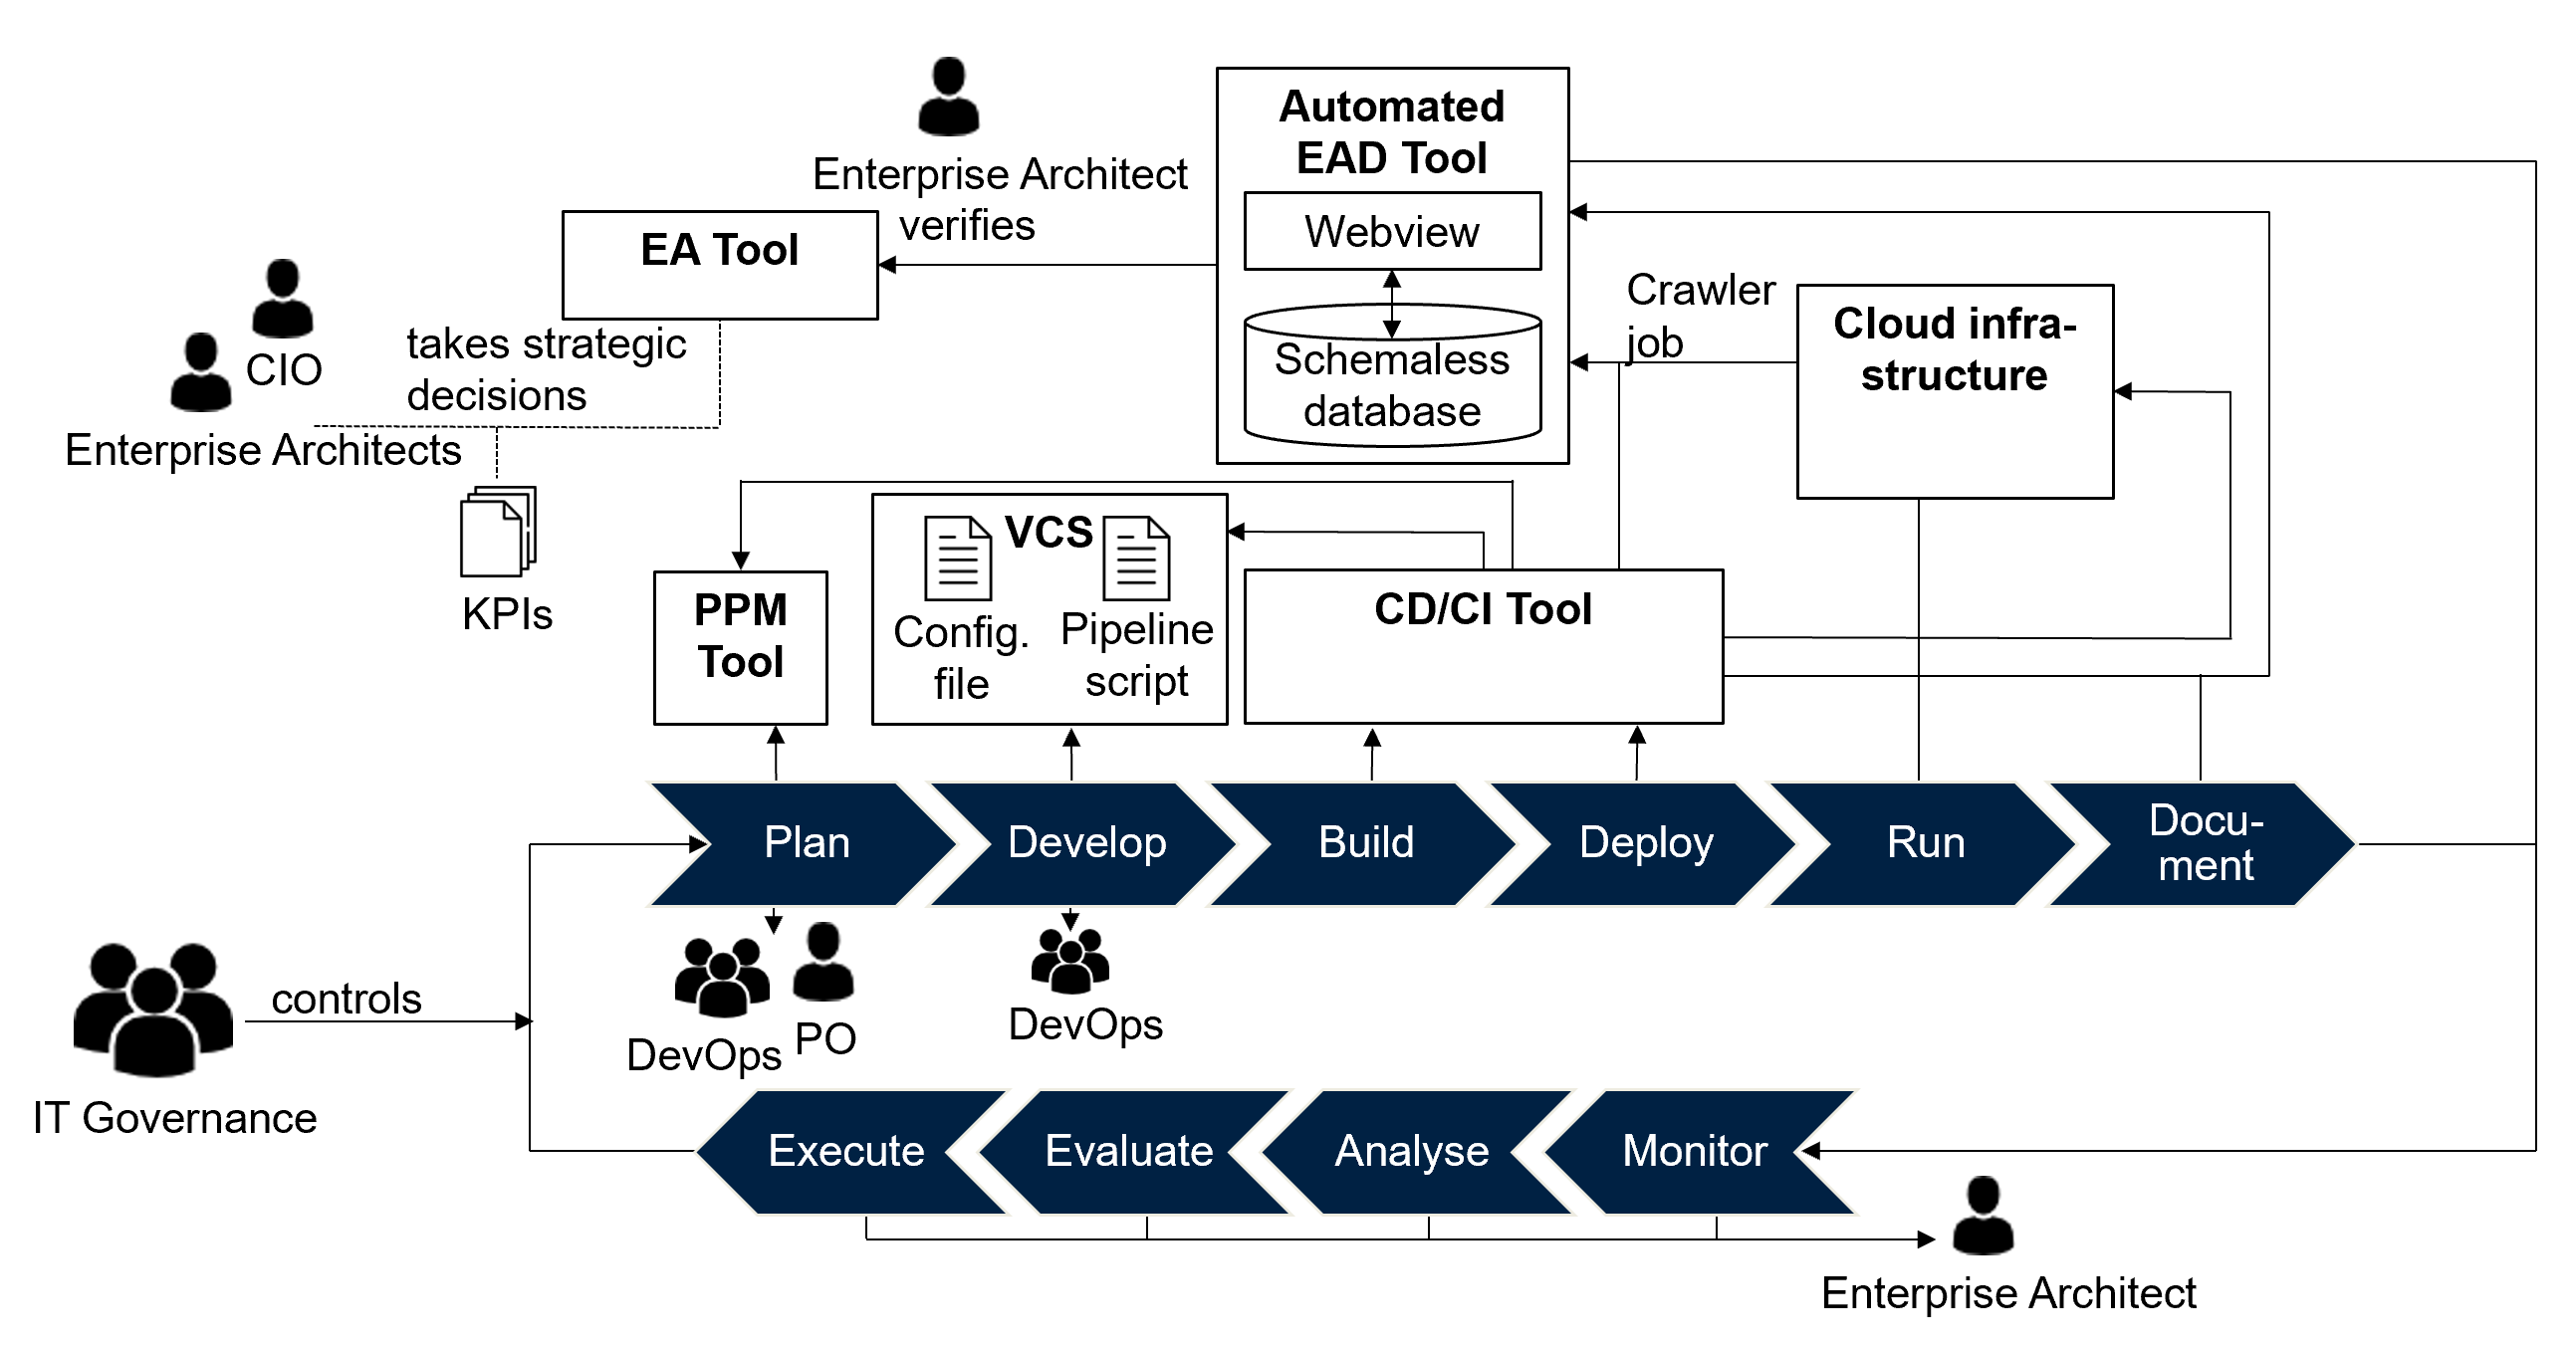
\includegraphics[width=1.0\textwidth]{figures/application-development-process.PNG}
  \caption{Application development process}
  \label{fig:application-development-process}
\end{figure}

Figure~\ref{fig:application-development-process} shows the application development process with its components and actors. The requirements and the process description are described in the following subsections.

\subsection{Requirements}\label{subsection:requirements}

To enable an automated documentation the fulfillment of the following requirements is needed:

\begin{itemize}
    \item A \textbf{predefined project structure} in the PPM tool
    \item The integration of a \textbf{configuration file}
    \item A \textbf{pipeline-script}
\end{itemize}
%Config file  in the repository containing the link to the PPM tool and other tools
%Pipelinescript
%Project structure
\subsubsection{Predefined project structure}

%In an agile development context PPM tools are used as an supporting tool.
A predefined project structure in the PPM tool and the fulfillment of the project structure enables the possibility to retrieve automatically the business information of the tool through the API. 
%agile and eam -> more dynamic eam. 
%structure attributes. domain, subdomain, product
%
The proposed structure for a project of this work is that every project should be at the same level as an application. Figure~\ref{fig:project-structure-mapping} shows proposed project structure and the alignment with archimate definitions.

\begin{figure}[htpb]
  \centering
  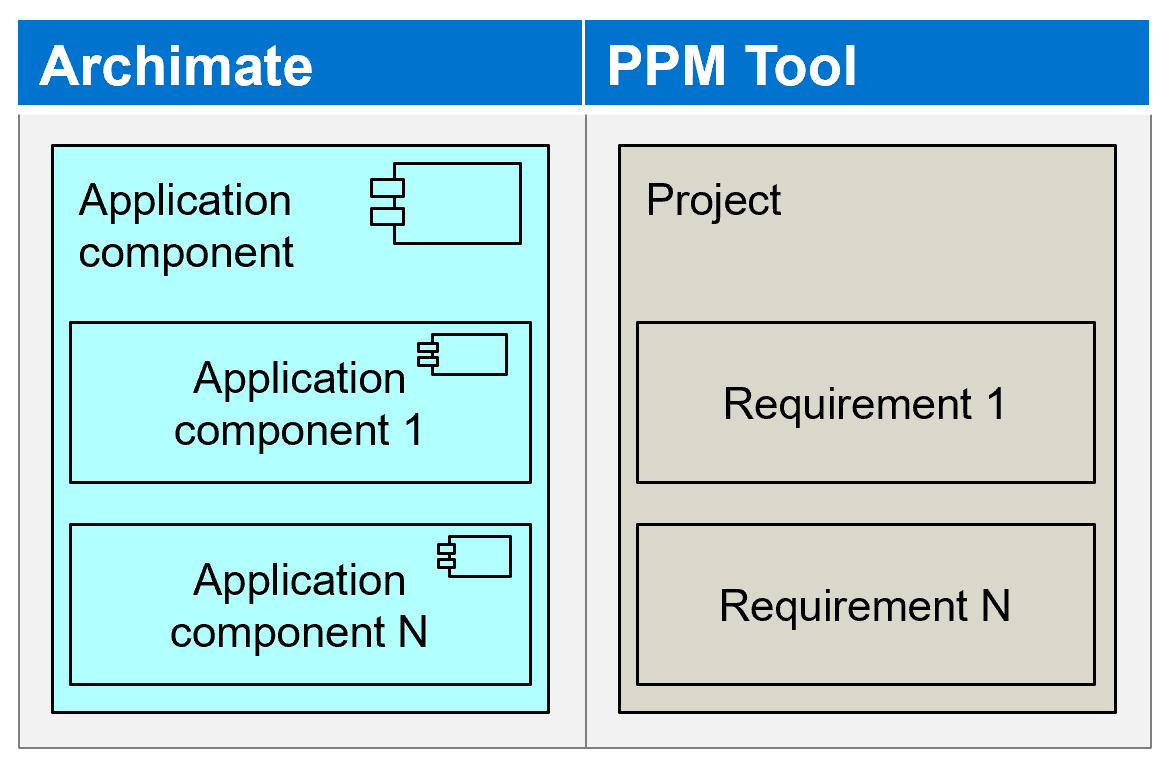
\includegraphics[width=0.8\textwidth]{figures/project-structure-mapping.PNG}
  \caption{Mapping of the the project structure}
  \label{fig:project-structure-mapping}
\end{figure}

The definition of an application component according to the archimate standard is: "An application component is defined as a modular, deployable, and replaceable part of a software system that encapsulates its behavior and data and exposes these through a set of interfaces." \hl{Archimate}

Since the archimate definition do not cover a definition for a parent application and a child application, the project has to be aligned to a parent application component. This application component as illustrated in figure~\ref{fig:project-structure-mapping} contains different application components. Each project requirement should be assigned to the children application components. Depending on the selected PPM tool, the business specific information can be stored at the project level or at the requirements level. In this approach the business information of the PPM tool is added at the requirements level. Each requirement should be assigned to a business domains and to a subdomain. The product information also stored at the requirements level corresponds to the parent application component. 
%The reason for storing the information at the requirements level is because the parent application can be used by different domains. 
The application owner would be mapped to the project owner in the PPM tool.

\subsubsection{Configuration file}

The addition of a configuration file in the repository has different functionalities. The main purpose for including a configuration file is that it contains a link to the PPM tool to retrieve the business information. The other purpose of the configuration file is to enable a federated enterprise architecture. The DevOps team manually maintain the links to other tools in this file. The added links can be stored as attributes of the applications in the metamodel of the tool enabling the linkage of the information enclosed by other tools.
%The DevOps team has to include all the links were the information about the application is contained. Linking other tools allows the possibility to s

\subsubsection{Pipeline-script}

A continuous delivery pipeline enables automation of the build and deployment pipeline and thus a documentation process can be integrated in the pipeline with no effort to enable the automation of EAD due to the reason that DevOps teams do not document minor changes. 
%Chen, Balalaie
In this manner the data quality attributes mentioned in table~\ref{tab:data-challenges} are automatically improved and documented. A manual separated documentation process is no longer necessary. Therefore the application development pipeline should integrate the documentation process within the continuous delivery pipeline. The idea is to include a similar mandatory script for each repository that enables the standardization of build, deployment and documentation process for every application. The intention of the script is that with small manual effort the DevOps team adapts the script. The adaptation of the script involves mainly the adjustments of authorization credentials. The script describes the flow of an artifact through different stages of the application pipeline. \hl{Hansen und Hacks 60-72}

\subsection{Process description}\label{subsection:processdescription}

The goal of this approach is to document EA relevant information automatically and to aggregate automatically business information to assign the application landscape to business domains (RQ1, RQ3). To ensure this automated aggregation of information the documentation process needs to cover the application development pipeline depicted in figure~\ref{fig:application-development-process}.

%Plan
The application development pipeline starts with the planning of a new software product. Therefore a PPM tool is needed. An automated documentation is only possible if the requirement of the project structure of subsection~\ref{subsection:requirements} is satisfied. 

When developing a new product/application the DevOps team must meet the two other requirements. The version control repository has to contain the configuration file with the link to the PPM tool and if possible other tools containing information about the product such as a wiki page for the product. The second requirements is that the pipeline script is included in the repository. 
This approach purposes a separate repository for each child application component. 
A deployment of the parent artifact is not needed because the deployment is usually separated into the deployment of small structures that communicate with other small structures. The automated documentation process of this approach is therefore included into the deployment of each application component. \hl{Bogner} 
%This approach documents Since the approach is about documenting applications running on cloud-based environments,  and thus a building process for a parent application component 
Decomposing an application into small structures like microservices and the development process of these lead to a quicker process of delivery to the customer to reduce the cycle time and release risks. \hl{Chen} Increasing the release frequency also leads to an accelerated time to market.\hl{Chen} Therefore the CD/CI tool starts the build process from the pipeline script included in the repository of the small structures.
Before building the artifact the pipeline script verifies that the configuration file is included into the repository and retrieves the business information for the specified application.

The tool should also include the deployment process because deployment failures rarely happen and this can be easy automated  within the pipeline script. \hl{Chen}

After the successfull deployment the pipeline script makes a call to the cloud infrastructure API to verify that the application is successfully running and to retrieve the runtime-behavior of the application.

As acknowledged by the survey conducted by Farwick et al. \hl{Farwick 2013} manual events can trigger an update of the documentation process. The build and deployment process can be used as triggers. Therefore the application development pipeline is used to trigger an automated EAD. \hl{Hansen und Hacks 60-72}. The documentation process pushes an aggregation of the collected EA information during the application pipeline to the automated EAD tool. This aggregation contains the business information from the PPM tool and the runtime-behavior of the application. The EAD tool contains a schemaless database with a REST API to facilitate the documentation. 

To update the runtime information of the applications running on cloud-based environments another process was defined in the CD/CI tool. The process is responsible for crawling the cloud infrastructure every certain time collecting and updating the runtime information in the automated EAD tool.

An uptodate EA information of cloud applications can be ensured and the manual effort for documentation processes can be eliminated. The inconsistency and redundancy of EA information retrieved from the cloud infrastructure can be removed through this process.
% because the documentation is always updated elimintating inconsistency and redundancy is not allowed t 
DevOps teams do not document smaller changes of an application in the EA tool. However, this process integrates the data from the DevOps toolchain automatically. Similar approaches call an are called "self-reporting architecture". \hl{Drews 2017}

The enteprise architect has the possibility to continuously monitor applications. It enables the detection of operational anomalies and performance related issues.\hl{Armin Balalaie and Abbas Heydarnoori} During the analyze and evaluation phase the enterprise architect can identify potential improvements from the monitored data. Afterwards, the enterprise architect executes the planned improvements while the IT Governance controls the fulfillment of policies and methods to ensure the alignment of the IT and the business goals. Based on that the IT Governance is also responsible for the management and monitoring of risks of IT resources.\hl{Meyer 2003}

Depending on the EA tool in place an export from the automated EAD tool to the EA tool is possible. A mapping between both tools is still needed. Once the mapping is implemented, the enterprise architect can verify the quality and consistency of the exported data in the EA tool. Since the automated EAD tool is only a middlelayer to aggregate information of different information sources the stakeholder will still take the decisions from the reportings and KPIs in the EA tool.

\section{Approach in usage scenario}\label{section:approach-usage-scenario}

To test the conceptual approach in a sample scenario the following tools described in subsection~\ref{subsection:toolselection} were used. The following figure~\ref{fig:Automated-EAD-process} shows the automated EAD process in the scenario with the selected tools.. The focus of this work is the process of an automated EAD from an application development pipeline. The process is explained in detail in subsection~\ref{subsection:scenarioprocessdescription}.

\subsection{Tool selection}\label{subsection:toolselection}

The following tools were used to test the conceptual approach of an automated documentation of Business Domain assignments and cloud application information from an application development pipeline.
\begin{itemize}
    \item The version control service Github is used as a web-based hosting for the code repositories.
    \item The open source automation server Jenkins is used to automate the application development process as a continuous integration and continuous delivery tool.
    \item To manage projects the Atlassian tool Jira is used. The tool enables an efficient Requirements Management for the project. \hl{Filion}
    \item The cloud infrastructure is enabled by the usage of the open source, multi-cloud application platform CloudFoundry.
    \item The existing open-source project Pivio is used as an automated EAD tool. The project is explained in detail in chapter~\ref{chapter:prototype implementation}
    \item The EA tool Iteraplan is used to test the approach. A lite version fo Iteraplan is available as a docker image. Iteraplan also allows the integration of other repositories through a public API.
\end{itemize}

\subsection{Fulfillment of requirements}\label{subsection:fulfillmentrequirements}

The definitions and components of the different tools selected for this approach need to be aligned. Figure~\ref{fig:tools-mapping} shows the mapping of definitions between the different tools and the alignment to the Archimate definition.

\begin{figure}[htpb]
  \centering
  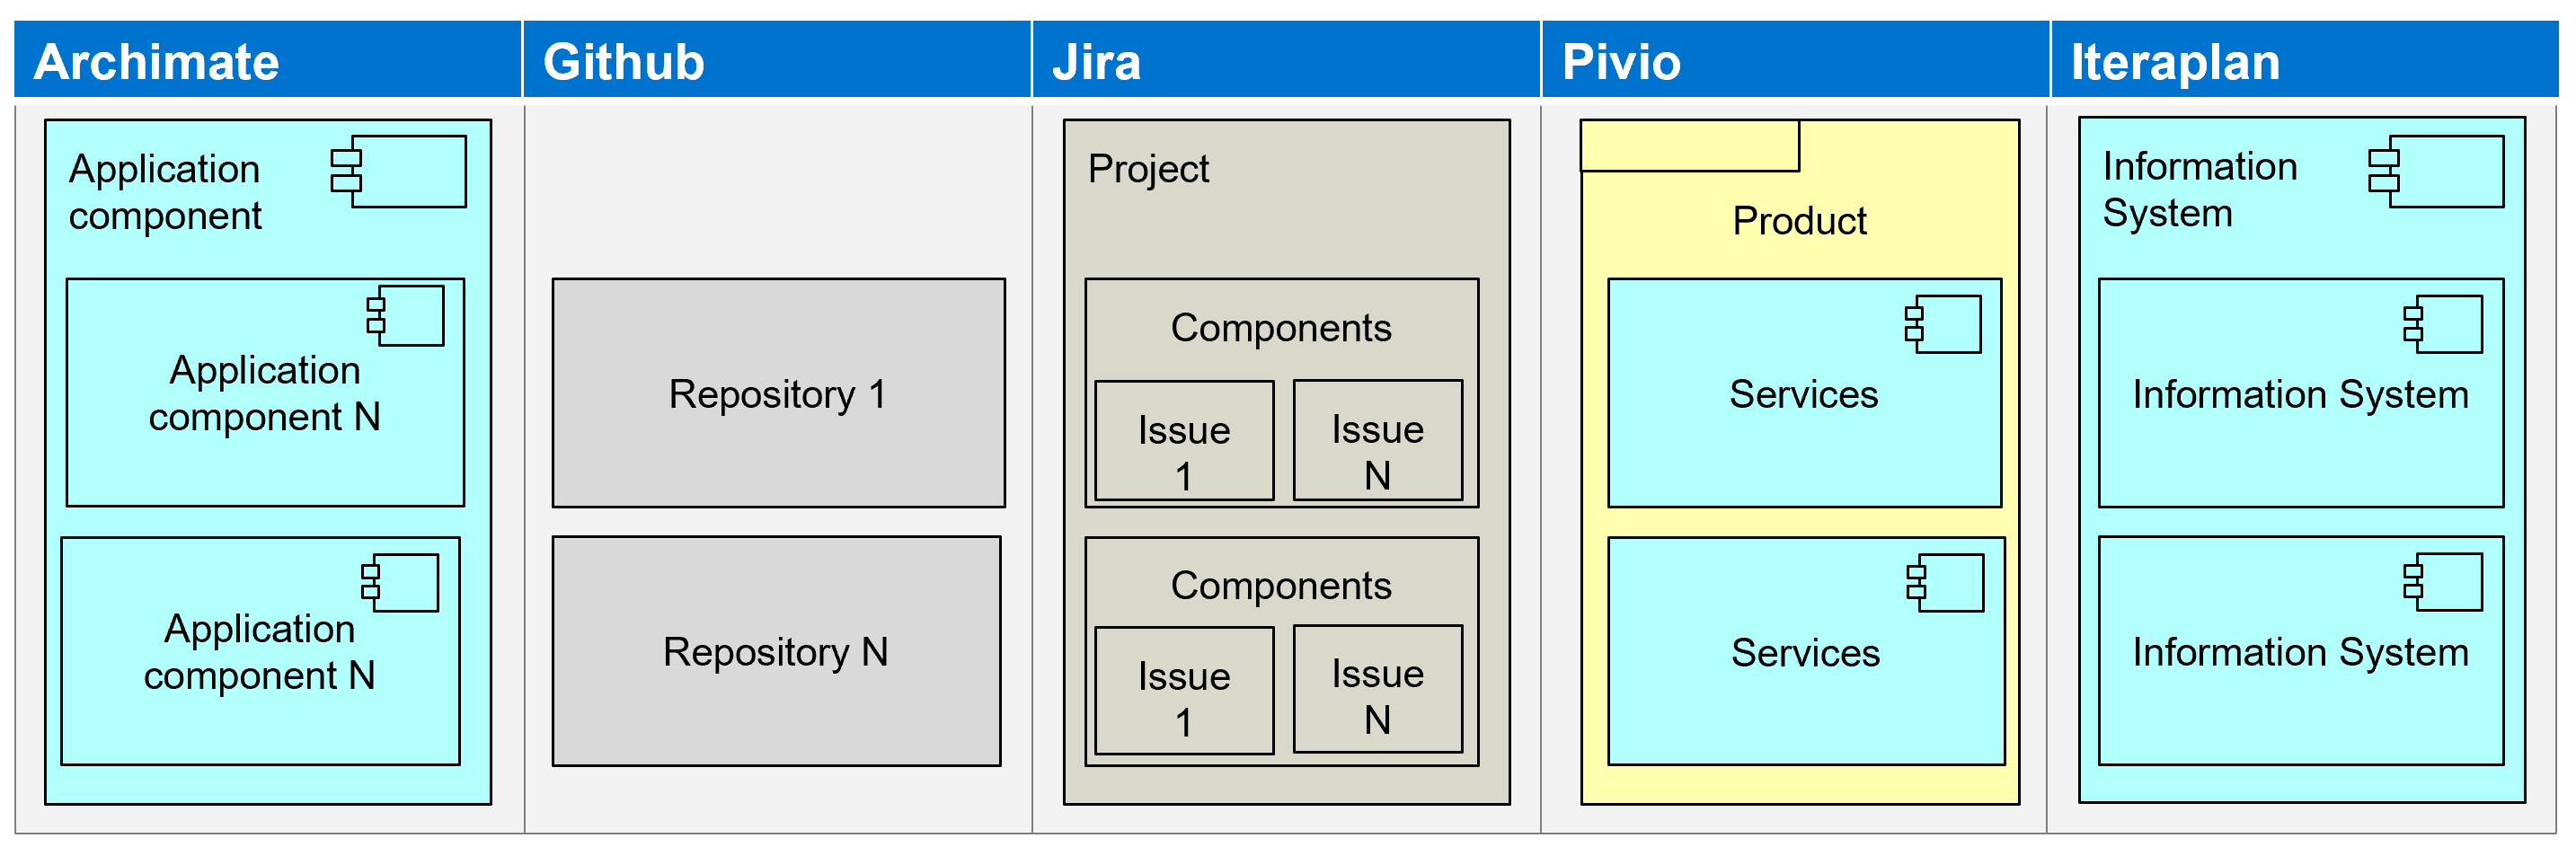
\includegraphics[width=1.0\textwidth]{figures/tools-mapping.PNG}
  \caption{Alignment of tools and Archimate}
  \label{fig:tools-mapping}
\end{figure}

For the application development process sample Springboot applications were developed in different repositories and the communication between these applications was implemented.

An example for the configuration file and the pipeline written in Groovy can be found in the appendix~\ref{chapter:appendix}

\subsection{Scenario process description}\label{subsection:scenarioprocessdescription}

\begin{figure}[htpb]
  \centering
  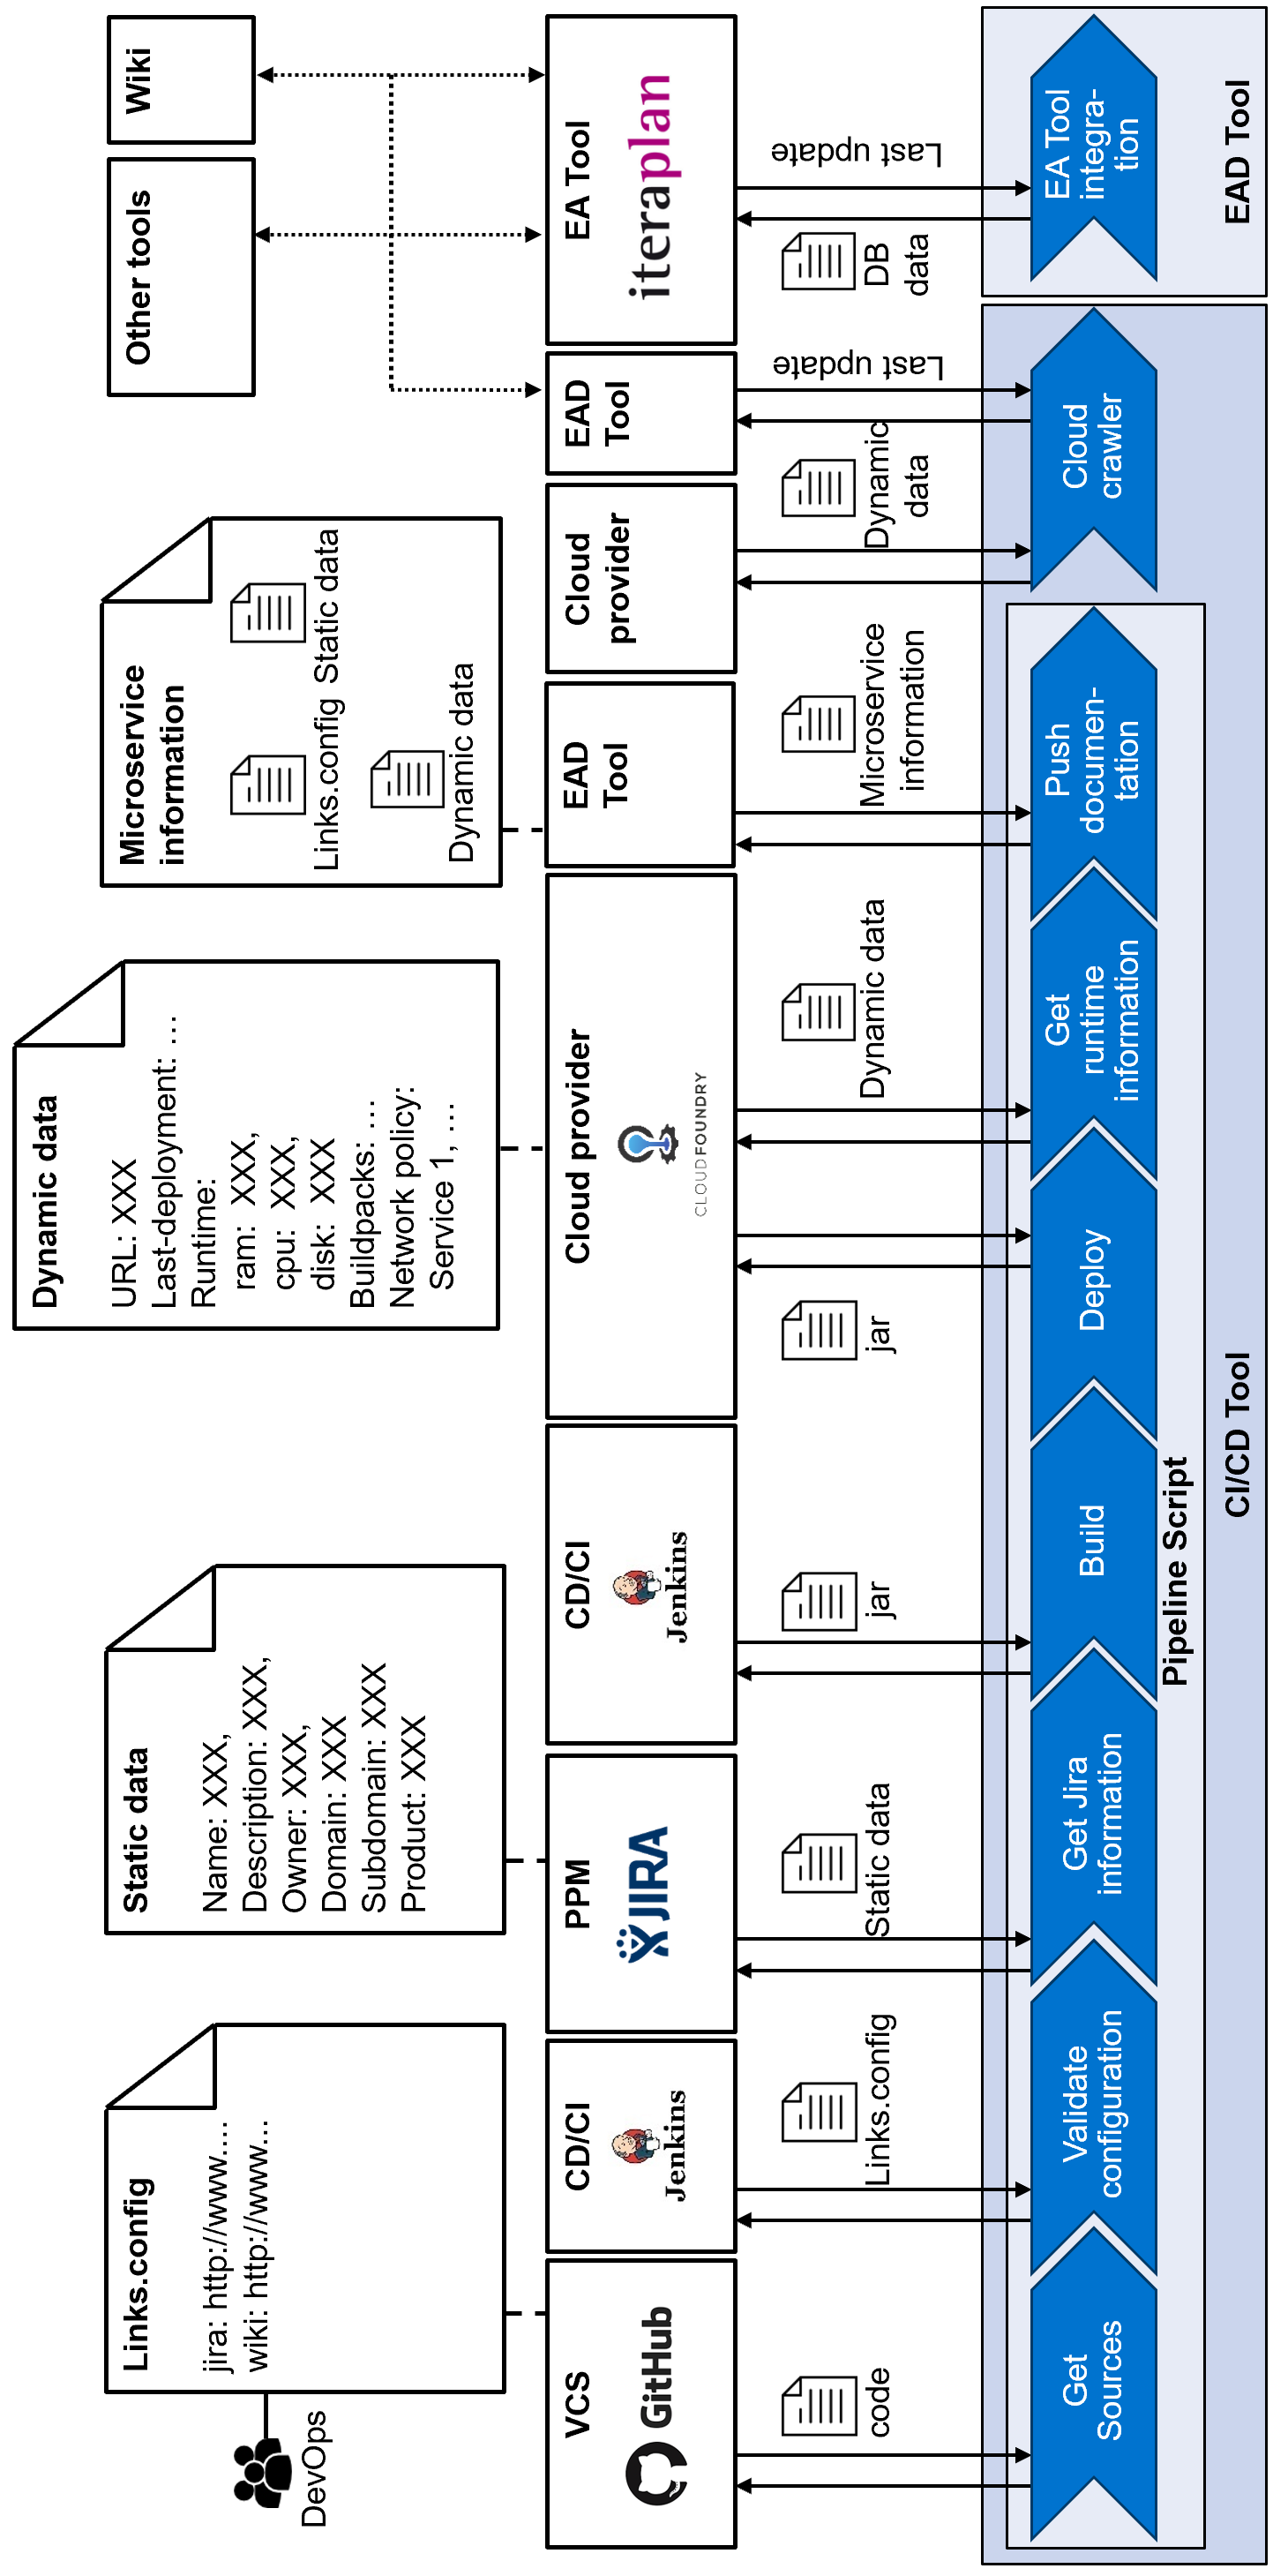
\includegraphics[width=0.65\textwidth]{figures/automated-ead-process-gedreht.png}
  \caption{Automated EAD process}
  \label{fig:Automated-EAD-process}
\end{figure}

To retrieve EA relevant information for an application running on a cloud-based environment the information is retrieved already during the application development pipeline and continuous integration tool. The EA relevant information collection process within the continuous integration tool is divided into two jobs. The first job is illustrated in figure~\ref{fig:Automated-EAD-process} as Groovy script. The second job is the crawler job which runs every certain time collecting the cloud and runtime information of the service. To enable the first job a groovy script has to be included into the repository of the version control service (requirement: pipeline script). The groovy-script represents the pipeline script. The pipeline shown in the picture above is divided into the following stages:

\subsubsection{Get sources}
This stage gets the latest code of the version control service. In this case the web-based hosting service for version control Github is used. The CD/CI Tool Jenkis downloads the repository locally. 

\subsubsection{Validate configuration}
To enable the retrievement of the business specific information and to enable the federated approach of the EA documentation, the configuration file has to be validated. The configuration file contains the links to other tools such a link to the PPM (Jira), a link to the CMDB, a link to the wiki, etc. The developers need to manually maintain and update the configuration file.

If the configuration file exists in the repository and it contains a link to the PPM tool in this case Jira the pipeline does not fail. Otherwise the pipeline fails to disable the inconsistent documentation regarding the business specific information.

\subsubsection{Get Jira information}\label{subsubsection:getjirainformation}
The stage "Get jira information" collects the business specific information. The stage is divided into two small parts to gather the information.

The first part makes a call to retrieve the information stored at the project level in jira. This information gets the project id, the project name, the project owner and the project description. 

The second part iterates through the issues assigned to the jira project. Every jira issue contains a standard field "component", which means to which child component of the parent application the issues is assigned to. Since jira does only allow to add customized fields at an issue level, each issue needs to contain the information of the domain, subdomain and product. To ensure the data quality attributes, the fields need to be mandatory when creating a new issue. The aggregated information of this part is stored at a global variable in the groovy script to be pushed at the documentation stage together with the information collected during the other stages.

As shown in the picture above this stage aggregates information from jira to the information being documented. Therefore every deployed aritfact can be aligned to a domain, subdomain and a product during the pipeline. This stage is the innovative part of the documentation process. Disabling the deployment of a service to the cloud before having the business-specific information of the service ensures that the EA information is consistent and complete. 

\subsubsection{Build}
Since the build stage together with the deployment stage are one of the most time consuming stages, the build and deployment stages where defined after collecting the business-specific information. The reason for this is that a completeness of the documentation is ensured. 
%As mentioned before collecting the business information during the documentation process takes less time than the build and deployment stage. To establish high quality of the EA information if the pipeline fails. 
The build-stage builds the downloaded code of the version control service with the commands defined in this stage. In this case Springboot applications were used to test the approach. Therefore Maven and/or Gradle commands were used to build the code. Depending on the size of the repository this stage may take some time.

\subsubsection{Deploy}
The deployment stage is also one of the most time consuming stages during this proposed pipeline. For the demonstration of this documentation process CloudFoundry is used as a multi-cloud application platform. This stage first connects to the cloud API endpoint with the credentials stored in the continuous delivery tool (jenkins). After authenticating, the organization and space of CloudFoundry are selected. The artifact is then pushed to the platform. If a manifest-yaml-file is defined in the repository, the specified information of that file is used for the cloud configuration. After executing the push command automatically, the platform downloads the buildpacks and software dependencies of the pushed artifact. The platform returns a message with the status of that the artifact. This means if the artifact was successfully or unsuccessfully deployed.

\subsubsection{Get Runtime Information}
Once the service was successfully deployed to the cloud the runtime information is retrieved. The information collected in this stage contains the following attributes:

\begin{itemize}
    \item Status of the services: is the service down or is the service running?
    \item How many instances of this services are running on the cloud?
    \item How much RAM does the service need of the predefined resources?
    \item How much CPU does the service consume?
    \item How much Disk of the predefined resources does the service expend?
    \item What buildpacks or software dependencies does the service require?
    \item What services does the deployed service communicate with?
\end{itemize}

The runtime information that can be gathered from the API may vary depending on the cloud infrastructure.

\subsubsection{Push Documentation}
During the pipeline the collected information of the individual stages are put in the same global variable of the script. The export of this variable is formatted as a json. As shown in the above picture the json contains the information of the configuration file, the business-specific information and the runtime information. This json is pushed to the tool with a simple HTTP-POST-Method.

\subsubsection{Cloud Crawler}
To updated the EA relevant information retrieved during the process, a crawler was implemented in the continuous delivery tool.The information update is depicted in figure \hl{XXX} as \textbf{Cloud Crawler}. The cloud crawler is a job in the CD tool that retrieves the runtime information of the cloud-based environment and updates the information in the \hl{solution tool}. The crawler job is divided in four stages. The following figure shows the cloud crawler job.

%bild von cloud crawler

\subsubsection{Get Pivio-App}

In this stage the job first retrieves a list of all artifacts listed in Pivio. 

Get Apps-List: 
In this stage the job gets a list of the artifacts that are hosted in the specified organization and space of the platform. This artifacts can be either running, stopped or crashed. Independently of the status of the service the platform API endpoint will return a complete list of the services.

%Erklärung warum liste aus tool und cloud

\subsubsection{Get individual Runtime Info}
Subsequently getting the list of all artifacts of the organization and space of the platform, this stage collects the individual runtime information. This stage iterates through the list of artifacts to retrieve the individual information of the them on the platform. The runtime information contains the attributes described in "Get Runtime Information". This is the most time consuming stage of the crawler job since the job has to retrieve the individual runtime information for each artifact.

\subsubsection{Push Documentation}
Ultimately the retrieved information of the individual services is pushed to Pivio to update the information of the already documented artifact to ensure an uptodate documentation.
The job is scheduled time-based. In the jenkins instance the crawler job is performed every 15 minutes.
%eampc: priorisierung von migrationen.
%eampc: aggregated architecture of enteprise oder cloud applikationen
